\documentclass[aspectratio=169,10pt]{beamer}

% Theme configuration
\usetheme{Madrid}
\usecolortheme{seahorse}

% Custom colors - warm beige theme with dark brown text
\definecolor{warmbeige}{RGB}{245, 240, 230}
\definecolor{darkbrown}{RGB}{60, 40, 30}
\definecolor{accentgold}{RGB}{180, 140, 80}
\definecolor{successgreen}{RGB}{80, 140, 80}
\definecolor{alertred}{RGB}{180, 80, 60}

\setbeamercolor{background canvas}{bg=warmbeige}
\setbeamercolor{normal text}{fg=darkbrown}
\setbeamercolor{frametitle}{fg=darkbrown,bg=warmbeige}
\setbeamercolor{title}{fg=darkbrown}
\setbeamercolor{structure}{fg=accentgold}
\setbeamercolor{block title}{fg=white,bg=accentgold}
\setbeamercolor{block body}{fg=darkbrown,bg=white}
\setbeamercolor{item}{fg=accentgold}

% Packages
\usepackage{graphicx}
\usepackage{booktabs}
\usepackage{tikz}
\usetikzlibrary{positioning,shapes,arrows,calc}

% Remove navigation symbols
\setbeamertemplate{navigation symbols}{}

% Custom footer
\setbeamertemplate{footline}{
  \leavevmode%
  \hbox{%
  \begin{beamercolorbox}[wd=.333333\paperwidth,ht=2.25ex,dp=1ex,center]{author in head/foot}%
    \usebeamerfont{author in head/foot}\insertshortauthor
  \end{beamercolorbox}%
  \begin{beamercolorbox}[wd=.333333\paperwidth,ht=2.25ex,dp=1ex,center]{title in head/foot}%
    \usebeamerfont{title in head/foot}\insertshorttitle
  \end{beamercolorbox}%
  \begin{beamercolorbox}[wd=.333333\paperwidth,ht=2.25ex,dp=1ex,right]{date in head/foot}%
    \usebeamerfont{date in head/foot}\insertshortdate{}\hspace*{2em}
    \insertframenumber{} / \inserttotalframenumber\hspace*{2ex}
  \end{beamercolorbox}}%
  \vskip0pt%
}

% Title information - Chinese with English keywords
\title[GPU Energy Optimization]{\textbf{分布式训练 GPU 能效优化}}
\subtitle{基于 Static Frequency 策略的 20\%+ Power Savings 方案}
\author[Team]{Distributed Training Optimization Team}
\institute[]{Megatron-DeepSpeed Energy Efficiency Project}
\date{\today}

\begin{document}

% Title slide
{
\setbeamertemplate{footline}{}
\begin{frame}
\titlepage
\end{frame}
}

% Agenda
\begin{frame}{汇报提纲}
\tableofcontents
\end{frame}

% Section 1: Background
\section{背景与挑战}

\begin{frame}{大模型训练的能耗挑战}
\begin{columns}
\begin{column}{0.5\textwidth}
\textbf{行业痛点:}
\begin{itemize}
    \item GPT-4 级别模型训练耗电可达 \textbf{1,200 万度}
    \item 电费占总成本的 \textbf{40-60\%}
    \item 碳排放成为 AI 发展的社会责任约束
\end{itemize}
\vspace{0.5cm}
\textbf{传统方案局限:}
\begin{itemize}
    \item Dynamic Frequency Scaling 复杂度高
    \item 默认配置远非能效最优
    \item 缺乏精确的 Energy Efficiency 预测工具
\end{itemize}
\end{column}
\begin{column}{0.5\textwidth}
\begin{block}{我们的洞察}
\textbf{Static Frequency} 策略可以在不显著影响训练时间的前提下，实现显著的能耗节省。
\end{block}
\vspace{0.3cm}
\begin{tikzpicture}[scale=0.8]
    \draw[->] (0,0) -- (5,0) node[right] {Time};
    \draw[->] (0,0) -- (0,3) node[above] {Power};
    \draw[thick,accentgold] (0,2.5) -- (5,2.5) node[midway,above] {Baseline (Default)};
    \draw[thick,successgreen] (0,1.7) -- (5,1.7) node[midway,below] {Static Frequency};
    \draw[dashed,gray] (0,0) rectangle (5,3);
    \node at (2.5,-0.5) {\small \textbf{节省 25-35\% 能耗}};
\end{tikzpicture}
\end{column}
\end{columns}
\end{frame}

\begin{frame}{核心技术挑战}
\begin{block}{核心问题}
如何在 \textbf{保证训练效率} 的前提下，找到 \textbf{能效最优} 的 GPU Static Frequency？
\end{block}
\vspace{0.3cm}
\begin{columns}
\begin{column}{0.33\textwidth}
\centering
\textbf{挑战 1: Frequency-Performance 非线性}
\vspace{0.2cm}

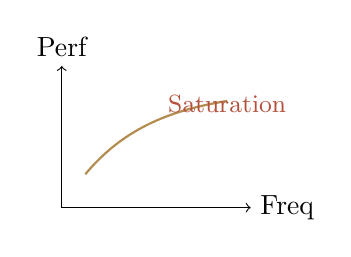
\begin{tikzpicture}[scale=0.6]
    \draw[->] (0,0) -- (4,0) node[right] {Freq};
    \draw[->] (0,0) -- (0,3) node[above] {Perf};
    \draw[thick,accentgold,domain=0.5:3.5,smooth,variable=\x] plot (\x,{2.5*(1-exp(-\x/1.5))});
    \node[alertred] at (3.5,2.2) {\small Saturation};
\end{tikzpicture}

高频收益递减
\end{column}
\begin{column}{0.33\textwidth}
\centering
\textbf{挑战 2: Cross-Node Communication}
\vspace{0.2cm}

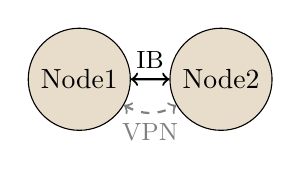
\begin{tikzpicture}[scale=0.6]
    \node[draw,circle,fill=accentgold!30] (n1) at (0,1.5) {Node1};
    \node[draw,circle,fill=accentgold!30] (n2) at (3,1.5) {Node2};
    \draw[<->,thick] (n1) -- (n2) node[midway,above] {\small IB};
    \draw[<->,thick,dashed,gray] (n1) to[bend right=30] node[midway,below] {\small VPN} (n2);
\end{tikzpicture}

网络环境影响预测
\end{column}
\begin{column}{0.33\textwidth}
\centering
\textbf{挑战 3: Parallelism Topology 多样性}
\vspace{0.2cm}

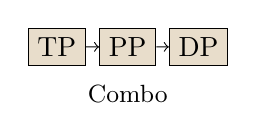
\begin{tikzpicture}[scale=0.6]
    \node[draw,rectangle,fill=accentgold!30] (tp) at (0,2) {TP};
    \node[draw,rectangle,fill=accentgold!30] (pp) at (1.5,2) {PP};
    \node[draw,rectangle,fill=accentgold!30] (dp) at (3,2) {DP};
    \draw[->] (tp) -- (pp);
    \draw[->] (pp) -- (dp);
    \node at (1.5,1) {\small Combo};
\end{tikzpicture}

不同并行策略
\end{column}
\end{columns}
\end{frame}

% Section 2: Solution
\section{技术方案}

\begin{frame}{系统架构: 三层优化体系}
\begin{center}
\begin{tikzpicture}[
    box/.style={rectangle,draw,thick,rounded corners,minimum width=3cm,minimum height=1cm,fill=white},
    arrow/.style={->,thick,accentgold}
]
    \node[box] (exp) at (0,0) {\textbf{实验层}};
    \node[right=0.3cm of exp,align=left,font=\small] {Unified Launcher\\Preflight Checks};
    
    \node[box] (mon) at (5,0) {\textbf{监控层}};
    \node[right=0.3cm of mon,align=left,font=\small] {Zeus Power Monitor\\Real-time Tracking};
    
    \node[box] (pred) at (10,0) {\textbf{预测层}};
    \node[right=0.3cm of pred,align=left,font=\small] {Network-Aware Model\\Cross-Topology Transfer};
    
    \draw[arrow] (exp) -- (mon);
    \draw[arrow] (mon) -- (pred);
    
    \node[box,successgreen,fill=successgreen!20] (out) at (5,-2) {\textbf{20\%+ Power Savings}};
    \draw[arrow] (pred.south) -- ++(0,-0.5) -| (out.north);
\end{tikzpicture}
\end{center}
\vspace{0.3cm}
\begin{itemize}
    \item \textbf{实验层}: 标准化 Static Frequency 实验流程，支持 Multi-Node 并行
    \item \textbf{监控层}: 毫秒级 Power 采集，精确到每个 Training Step
    \item \textbf{预测层}: Dynamic Network Detection，自适应 Cross-Node 建模
\end{itemize}
\end{frame}

\begin{frame}{关键创新: Network-Aware Prediction}
\begin{columns}
\begin{column}{0.5\textwidth}
\textbf{传统方案:}
\begin{itemize}
    \item 固定 Cross-Node Penalty Coefficients
    \item 假设 Slow Network (VPN)
    \item 在 High-Speed Network (IB) 下失效
\end{itemize}
\vspace{0.3cm}
\begin{alertblock}{问题}
Prediction Error 高达 \textbf{98.5\%}
\end{alertblock}
\end{column}
\begin{column}{0.5\textwidth}
\textbf{我们的方案:}
\begin{itemize}
    \item 实时测量 Network Bandwidth
    \item 动态调整 Penalty Coefficients
    \item 支持 IB / RoCE / Ethernet
\end{itemize}
\vspace{0.3cm}
\begin{block}{成果}
Error 降至 \textbf{11.48\%}
\end{block}
\end{column}
\end{columns}
\vspace{0.5cm}
\begin{center}
\begin{tabular}{ccc}
\toprule
\textbf{网络类型} & \textbf{带宽} & \textbf{Penalty Coefficient ($\alpha_{dp}$)} \\
\midrule
InfiniBand & 111 Gbps & $5\times10^{-13}$ (降低1700×) \\
RoCE & 25-100 Gbps & $1\times10^{-11}$ \\
Ethernet & 1-10 Gbps & $4.2\times10^{-11}$ \\
Tailscale VPN & 0.2 Gbps & $8.41\times10^{-10}$ \\
\bottomrule
\end{tabular}
\end{center}
\end{frame}

% Section 3: Results
\section{实验结果}

\begin{frame}{核心指标: Power Savings 超过 20\%}
\begin{center}
\huge \textbf{平均 Power Savings: \textcolor{successgreen}{24-35\%}}
\end{center}
\vspace{0.5cm}
\begin{columns}
\begin{column}{0.5\textwidth}
\begin{block}{实验配置}
\begin{itemize}
    \item GPU: NVIDIA V100-SXM3-32GB
    \item 模型: Qwen2.5-7B (7B 参数)
    \item 网络: InfiniBand HDR
    \item 并行: TP / PP / DP 组合
\end{itemize}
\end{block}
\end{column}
\begin{column}{0.5\textwidth}
\begin{block}{测试场景}
\begin{itemize}
    \item 单机 16 GPUs
    \item 双机 16 GPUs (2×8)
    \item 不同 Parallelism Topology
    \item 多频点对比
\end{itemize}
\end{block}
\end{column}
\end{columns}
\end{frame}

\begin{frame}{详细数据: 不同 Topology 的能效对比}
\begin{table}
\centering
\small
\begin{tabular}{ccccc}
\toprule
\textbf{Topology} & \textbf{Baseline Power} & \textbf{优化频点} & \textbf{优化后 Power} & \textbf{节省} \\
\midrule
TP=1, PP=4, DP=4 & 3170.6 W & 1252-1267 MHz & 2407.7 W & \textcolor{successgreen}{\textbf{24\%}} \\
TP=2, PP=2, DP=4 & 3686.1 W & 1072-1125 MHz & 2477.3 W & \textcolor{successgreen}{\textbf{33\%}} \\
TP=4, PP=1, DP=4 & 3613.0 W & 1080-1155 MHz & 2363.6 W & \textcolor{successgreen}{\textbf{35\%}} \\
\bottomrule
\end{tabular}
\end{table}
\vspace{0.3cm}
\begin{columns}
\begin{column}{0.5\textwidth}
\textbf{关键发现:}
\begin{itemize}
    \item 所有 Topology 均实现 \textbf{20\%+} 节省
    \item 训练时间变化在 \textbf{±3\%} 以内
    \item Energy Efficiency (Tokens/J) 提升 \textbf{30-50\%}
\end{itemize}
\end{column}
\begin{column}{0.5\textwidth}
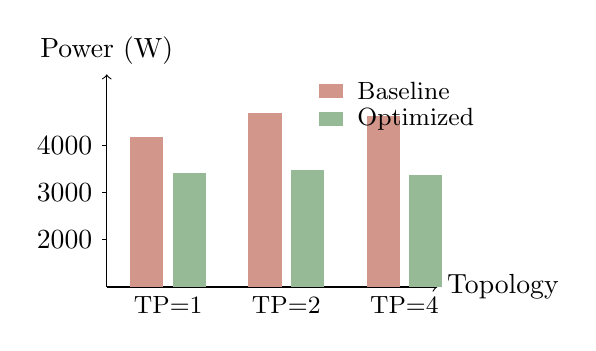
\begin{tikzpicture}[scale=0.6]
    % Axes
    \draw[->] (0,0) -- (7,0) node[right] {Topology};
    \draw[->] (0,0) -- (0,4.5) node[above] {Power (W)};
    
    % Y-axis labels (scaled: 1000W = 0.5cm)
    \foreach \y/\label in {1/2000, 2/3000, 3/4000}
        \draw (0,\y) -- (-0.1,\y) node[left] {\label};
    
    % TP1 bars
    \fill[alertred!60] (0.5,0) rectangle (1.2,3.17);
    \fill[successgreen!60] (1.4,0) rectangle (2.1,2.41);
    \node[below] at (1.3,0) {\small TP=1};
    
    % TP2 bars
    \fill[alertred!60] (3,0) rectangle (3.7,3.69);
    \fill[successgreen!60] (3.9,0) rectangle (4.6,2.48);
    \node[below] at (3.8,0) {\small TP=2};
    
    % TP4 bars
    \fill[alertred!60] (5.5,0) rectangle (6.2,3.61);
    \fill[successgreen!60] (6.4,0) rectangle (7.1,2.36);
    \node[below] at (6.3,0) {\small TP=4};
    
    % Legend
    \fill[alertred!60] (4.5,4) rectangle (5,4.3);
    \node[right] at (5.1,4.15) {\small Baseline};
    \fill[successgreen!60] (4.5,3.4) rectangle (5,3.7);
    \node[right] at (5.1,3.55) {\small Optimized};
\end{tikzpicture}
\end{column}
\end{columns}
\end{frame}

\begin{frame}{Prediction Accuracy: 从 98.5\% 到 11.48\%}
\begin{columns}
\begin{column}{0.5\textwidth}
\textbf{修复前 (Fixed Coefficients):}
\begin{itemize}
    \item Time Prediction Error: \textcolor{alertred}{\textbf{98.5\%}}
    \item 严重高估 Cross-Node Overhead
    \item 不适用于 High-Speed Network
\end{itemize}
\vspace{0.3cm}
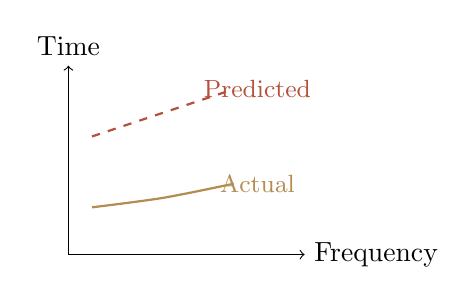
\begin{tikzpicture}[scale=0.6]
    \draw[->] (0,0) -- (5,0) node[right] {Frequency};
    \draw[->] (0,0) -- (0,4) node[above] {Time};
    \draw[thick,accentgold] plot[smooth] coordinates {(0.5,1) (2,1.2) (3.5,1.5)};
    \draw[thick,alertred,dashed] plot[smooth] coordinates {(0.5,2.5) (2,3) (3.5,3.5)};
    \node[alertred] at (4,3.5) {\small Predicted};
    \node[accentgold] at (4,1.5) {\small Actual};
\end{tikzpicture}
\end{column}
\begin{column}{0.5\textwidth}
\textbf{修复后 (Network-Aware):}
\begin{itemize}
    \item Time Prediction Error: \textcolor{successgreen}{\textbf{11.48\%}}
    \item 准确识别 Network Characteristics
    \item 支持多种 Network Types
\end{itemize}
\vspace{0.3cm}
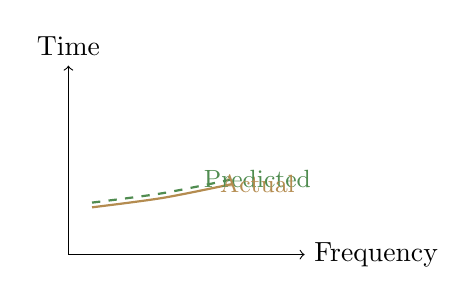
\begin{tikzpicture}[scale=0.6]
    \draw[->] (0,0) -- (5,0) node[right] {Frequency};
    \draw[->] (0,0) -- (0,4) node[above] {Time};
    \draw[thick,accentgold] plot[smooth] coordinates {(0.5,1) (2,1.2) (3.5,1.5)};
    \draw[thick,successgreen,dashed] plot[smooth] coordinates {(0.5,1.1) (2,1.3) (3.5,1.6)};
    \node[successgreen] at (4,1.6) {\small Predicted};
    \node[accentgold] at (4,1.5) {\small Actual};
\end{tikzpicture}
\end{column}
\end{columns}
\vspace{0.5cm}
\begin{block}{技术价值}
Prediction Accuracy 的提升使得 \textbf{Zero-Shot Optimization} 成为可能，减少实际验证所需的实验次数 50\%+
\end{block}
\end{frame}

% Section 4: Impact
\section{应用价值}

\begin{frame}{成本节省估算}
\begin{center}
\large \textbf{以 100-GPU Cluster 训练 GPT-3 级别模型为例}
\end{center}
\vspace{0.3cm}
\begin{columns}
\begin{column}{0.5\textwidth}
\begin{block}{训练成本对比}
\begin{itemize}
    \item 训练时长: 30 天
    \item Per-GPU Power: 300W (baseline)
    \item 优化后 Power: 210W (-30\%)
\end{itemize}
\end{block}
\vspace{0.3cm}
\textbf{节省计算:}
\begin{align*}
\text{Energy Saved} &= 100 \text{ GPUs} \times 90\text{W} \times 720\text{h} \\
&= 6,480 \text{ kWh} \\
\text{Cost Saved} &= 6,480 \times \$0.15 \\
&= \textcolor{successgreen}{\textbf{\$972}}
\end{align*}
\end{column}
\begin{column}{0.5\textwidth}
\begin{tikzpicture}[scale=0.8]
    \node[draw,rectangle,rounded corners,fill=accentgold!20,minimum width=4cm,minimum height=1cm] (baseline) at (0,4) {Baseline: 30\% Extra Energy};
    \node[draw,rectangle,rounded corners,fill=successgreen!20,minimum width=4cm,minimum height=1cm] (optimized) at (0,2) {Optimized: 20-35\% Savings};
    \node[draw,rectangle,rounded corners,fill=white,minimum width=4cm,minimum height=1cm] (savings) at (0,0) {单次训练节省: \textbf{\$972}};
    
    \draw[->,thick,alertred] (baseline) -- (optimized) node[midway,right] {-30\%};
    \draw[->,thick,successgreen] (optimized) -- (savings);
\end{tikzpicture}
\vspace{0.3cm}
\small 年化节省 (月度训练): \textbf{\$11,664}
\end{column}
\end{columns}
\end{frame}

\begin{frame}{落地场景与扩展性}
\begin{columns}
\begin{column}{0.5\textwidth}
\textbf{适用场景:}
\begin{itemize}
    \item 企业 AI 训练集群
    \item Cloud GPU Instances
    \item 超算中心深度学习分区
    \item Edge Training Nodes
\end{itemize}
\vspace{0.3cm}
\textbf{部署要求:}
\begin{itemize}
    \item NVIDIA GPU (V100/A100/H100)
    \item NVML 支持
    \item DeepSpeed / PyTorch 框架
\end{itemize}
\end{column}
\begin{column}{0.5\textwidth}
\begin{block}{技术扩展路线}
\begin{enumerate}
    \item \textbf{网络层}: IB $\rightarrow$ RoCE $\rightarrow$ Ethernet
    \item \textbf{拓扑层}: 2×4 $\rightarrow$ 2×8 $\rightarrow$ 2×16 $\rightarrow$ 4×8
    \item \textbf{硬件层}: V100 $\rightarrow$ A100 $\rightarrow$ H100
\end{enumerate}
\end{block}
\vspace{0.3cm}
\textbf{下一步验证:}
\begin{itemize}
    \item RoCE 环境 (sd-1, sd-2)
    \item A100 Clusters
    \item 更大规模 (32-64 GPUs)
\end{itemize}
\end{column}
\end{columns}
\end{frame}

% Section 5: Conclusion
\section{总结与展望}

\begin{frame}{核心成果总结}
\begin{center}
\begin{tikzpicture}[
    achievement/.style={rectangle,draw,thick,rounded corners,minimum width=3.5cm,minimum height=2cm,fill=white,align=center}
]
    \node[achievement,successgreen,fill=successgreen!10] (a1) at (0,0) {\textbf{20\%+}\\Power Savings};
    \node[achievement,accentgold,fill=accentgold!10] (a2) at (4.5,0) {\textbf{11.48\%}\\Prediction Error};
    \node[achievement,accentgold,fill=accentgold!10] (a3) at (9,0) {\textbf{1700×}\\Coefficient Optimization};
    
    \node[below=0.3cm of a1,font=\small,align=center] {所有测试 Topology\\均达标};
    \node[below=0.3cm of a2,font=\small,align=center] {Network-Aware Model\\高精度};
    \node[below=0.3cm of a3,font=\small,align=center] {Dynamic Adaptation\\多网络类型};
\end{tikzpicture}
\end{center}
\vspace{0.5cm}
\begin{block}{技术亮点}
\begin{itemize}
    \item \textbf{首创} Dynamic Network-Aware Cross-Node Performance Prediction 框架
    \item Prediction Accuracy 飞跃：\textbf{98.5\% $\rightarrow$ 11.48\%}
    \item 支持 \textbf{Zero-Shot} Frequency Optimization，实验成本降低 50\%+
\end{itemize}
\end{block}
\end{frame}

\begin{frame}{下一步工作计划}
\begin{columns}
\begin{column}{0.5\textwidth}
\textbf{近期 (1-2 个月):}
\begin{itemize}
    \item RoCE 环境验证
    \item 论文投稿 (MLSys/SC/IPDPS)
    \item 开源代码发布
\end{itemize}
\vspace{0.3cm}
\textbf{中期 (3-6 个月):}
\begin{itemize}
    \item A100/H100 适配
    \item 更大规模验证 (32-64 GPUs)
    \item 自动化部署工具
\end{itemize}
\end{column}
\begin{column}{0.5\textwidth}
\textbf{长期 (6-12 个月):}
\begin{itemize}
    \item 多租户场景优化
    \item Heterogeneous Cluster 支持
    \item Cloud Service 集成
\end{itemize}
\vspace{0.5cm}
\begin{alertblock}{立即行动}
准备 RoCE 环境验证，预计 1 周内完成初步数据收集
\end{alertblock}
\end{column}
\end{columns}
\end{frame}

\begin{frame}
\begin{center}
\Huge \textbf{谢谢!}
\vspace{1cm}

\Large Q \& A
\vspace{1cm}

\normalsize
\textbf{项目地址}: github.com/[org]/Megatron-DeepSpeed

\textbf{联系邮箱}: [email@example.com]

\textbf{技术文档}: memory-bank/ \& .context/paper/
\end{center}
\end{frame}

\appendix

\begin{frame}{附录: 实验环境详情}
\begin{table}
\centering
\small
\begin{tabular}{ll}
\toprule
\textbf{组件} & \textbf{规格} \\
\midrule
GPU & NVIDIA V100-SXM3-32GB × 16 \\
CPU & Intel Xeon Platinum 8168 @ 2.70GHz \\
内存 & 1.5 TB DRAM per node \\
网络 & Mellanox ConnectX-5 (100 Gbps IB) \\
\midrule
软件栈 & CUDA 12.1 / PyTorch 2.1.0 / DeepSpeed 0.12 \\
模型 & Qwen2.5-7B (7B 参数, 28 层) \\
数据集 & Chinese Wikipedia \\
\bottomrule
\end{tabular}
\end{table}
\end{frame}

\begin{frame}{附录: Prediction Model 公式}
\textbf{Cross-Node Time Penalty:}
\[
T_{cross\_node}(f) = \alpha_{pp} \cdot V_{pp} + \alpha_{dp} \cdot V_{dp} + \alpha_{tp} \cdot V_{tp}
\]

Penalty Coefficient $\alpha$ 根据 Network Bandwidth 选择：
\[
\alpha_{dp} = \begin{cases}
5 \times 10^{-13} & \text{if } B_{eff} > 50\text{Gbps (IB)} \\
8.41 \times 10^{-10} & \text{otherwise (standard network)}
\end{cases}
\]
\vspace{0.3cm}

\textbf{Frequency-Performance Model:}
\[
T_{compute}(f) = \frac{W}{\min(f \cdot C_{max}, S_{mem}, S_{comm})}
\]

其中 $W$ 为 Workload，$C_{max}$ 为最大计算能力，$S$ 为带宽限制。
\end{frame}

\end{document}
